\documentclass[10pt,oneside,slovak,a4paper]{article}
\usepackage{float}
\usepackage[slovak]{babel}
\usepackage[IL2]{fontenc}
\usepackage[utf8]{inputenc}
\usepackage{graphicx}
\usepackage{url}
\usepackage{hyperref}

\usepackage{cite}

\pagestyle{headings}

\title{Obmedzení už len predstavivosťou\thanks{Semestrálny projekt v predmete Metódy inžinierskej práce, ak. rok 2022/23, vedenie: Zuzana Špitálová}}

\author{Tomáš Lasak\\[2pt]
	{\small Slovenská technická univerzita v Bratislave}\\
	{\small Fakulta informatiky a informačných technológií}\\
	{\small \texttt{xlasak@stuba.sk}}
	}

\date{\small 30. Október 2022}

\begin{document}

\maketitle

\paragraph{Inžinierska práca v informatike a písanie technického textu.}

Nie som si úplne istý, či cieľ prezentácie mal mať taký dopad na poslucháčov aký mal.
Začiatok bol zaujímavý, ale prišlo mi to moc vecne a nevedel som si tento postup moc predstaviť.
Myslím si, že by pomohli nejaké obrázky ako príklady, ktoré sa zaryjú v pamäti.
Na druhú stranu, po nejakom čase, kedy prezentácia a výklad pôsobil dosť uvoľnene prišla veľká zmena.
Skočilo sa príliš rýchlo na vecnú časť.
Mám pocit, že publikum si takto nemalo možnosť ako niečo zobrať z prvej časti, čo mi príde individuálne dôležitejšia na sebarozvoj.

\paragraph{Prezentácia: slajdy a prednes.}

K prezentácii by som mal niekoľko pripomienok.
V prvom rade to nemyslím zle, no mnoho informácií bolo reprezentovných inak akoby sa po správnosti malo.
Celá téma o prezentáciach ako celok mi príde dosť individuálna od rôznej problematiky.
Vzhľadom na to, že sa pracuje s ľuďmi, ktorí nemusia mať grafické základy mohli by to zle pochopiť.
Celkom som zostal zaskočený, že predmet má striktné podmienky pri výbere nástroja pre prezentáciu.
Taktiež dosť individuálne, pretože som mal pocit, že predmet tu je na to, aby študentov zoznámil a ukázal im akúsi možnú cestu,
kde ľudí, kde ako príklad použijem seba, trochu obmedzil.

\paragraph{Technológia a ľudia: Scrum.}

Zaujímava téma. Príjemné na počúvanie a myšlienka ukázať študentom, ako "modernejšie" firmi pracujú, bola super.
Prezentácia šla dosť plynulo a výklad bol zaujímavý.
Mnoho vecí, sa dá uplatniť aj v iných oblastiach, kde sa pracuje s ľuďmi.
Dokonca aj pri riešení problémov, z každodenného života, alebo školy.

\pagebreak

\begin{abstract}

	Myslím si, že je dôležité veci chápať predtým ako s nimi začneme pracovať. Preto si jednotlivé celky najskôr predstavíme a do istej časti rozoberieme.
	Začneme základnými princípmi počítača. Ďalej sa vrhneme už na samotnú prácu a využitie technológií, čo nám svet prináša.
	Celé to bude zamerané na jednoduchosť témy, myšlienkou bude poukázať na to, že vytvoriť v dnešnej dobe zaujímavú, až dych berúcu aplikáciu, alebo len 3D interakciu, nie je ťažké.
	Jediný háčik je sa schováva v osvojení si technológií na túto tvorbu.
	No ako už bolo spomínané, nikdy to nebolo ľahšie ako teraz, dokonca to vyzerá tak, že už sa hýbeme iba ľahším a ľahším smerom.
	To so sebou prináša aj záujem a s rastúcim záujmom však rastie aj konkurencia a stáva sa z toho závod nami individuálne vnímaní.
	Pre niekoho vrátane mňa môže ísť o hru, kde vašim cieľom je predstaviť niečo obrovské a po dosiahnutí úspechu ho opakovať a stále dookola.
	Preto som sa rozhodol napísať ako vnímam tento vývoj ja svojimi očami, a kam si myslím, že smerujeme.
	Aj pre prípad, že za sebou nemáte toľko skúseností, snažil som sa opisovať oblasti viacej abstraktne, aby bolo možné si to aspoň predstaviť a pohrať sa s predstavivosťou, čo je aj hlavná myšlienka celého projektu.
	Nenechať sa obmedziť. Nakoniec, v závere ešte spomeniem užitočné zdroje, postupy a môj názor na vec.

\end{abstract}

\section{Technológie}

\subsection{Procesor}

“V dnešnej dobe sa stretávame s dvomi typmi procesorov v počítačoch, známe pod názvami CPU a GPU. Už takmer všetky počítače obsahujú najmenej dva procesory.” \cite{Graphics-programming}
Každý z nich je unikátny a vhodný na rôzne druhy výpočtov. Nás bude zaujímať hlavne GPU. GPU inak ako grafický procesor zvyčajne už dnes umiestnený v grafickej karte.
Tento procesor je zaujímavý svojou výkonnosťou.
Na rozdiel od CPU, GPU pracuje s množstvo menších výpočtov, no oveľa rýchlejšie, zodpovedá za vykonávanie a počítanie matematických operácií, čím výkonnejší procesor, tým sú výpočty rýchlejšie.
Tieto zmeny vie aplikovať do grafického rozhrania. (link1) To je nám ako užívateľom bližšie, pretože zmenu vieme zaznamenať vizuálne.

\subsection{OpenGL}

Aby sme boli schopný vytvoriť 3D interakciu do nášho programu, potrebujeme túto inštrukciu dostať do grafického procesora.
Našťastie pre nás existujú spôsoby, ako posielať inštrukcie a komunikovať s grafickým procesorom.
“Dnešným štandardom komunikácie s grafickým procesorom je OpenGL. OpenGL je moderná multiplatformová knižnica na prepojenie sa s GPU za účelom vykresľovania 3D grafiky v reálnom čase.” \cite{Graphics-openGL}
Jej súčasťou je mnoho preddefinovaných funkcii pre prácu s 2D a 3D. Pre začiatok je ideálne mať nejaké základy programovania.
No pre prípad, že skúsenosti nemáme, tak najjednoduchšie je si predstaviť programovanie ako veľkú sa príkazov.
Pri písaní sa niekedy sa dostaneme do situácie, že sa začneme v inštrukciách opakovať, v takom prípade obalíme príkazy do blokov, nazývané funkcie, tieto funkcie neskôr vieme vyvolávať ako potrebujeme.
Pojem knižnica v programovaní si vieme predstaviť ako sadu týchto funkcii. Najväčšiu časť OpenGL knižnice zaberajú funkcie pracujúce s matematickými výpočtami zväčša sa týkajúce lineárnej algebry.

\subsection{WebGL}

Webové prehliadače sú žiaľ limitované a priamy prístup ku knižnici OpenGL. Je tu však alternatívna knižnica nazývaná WebGL, postavená na knižnici OpenGL.
WebGL je rovnako grafická knižnica na vykresľovanie 2D a 3D grafiky, s rozdielom, že len v prostredí webového prehliadača.
To znamená, že taktiež aj aplikácie vytvorené v tomto prostredí zobrazujúce 2D alebo 3D interakcie, budú používať WebGL.
Pomocou JavaScriptu a html vieme využiť WebGL funkcie. Html tvorí štruktúru stránky a elementy v ňom reprezentujú obsah stránky.
Element ktorý potrebujeme v našom prípade je canvas, je to element určený na prezentovanie 2D a 3D grafického obsahu. JavaScript je programovací jazyk, ktorý dodáva webovej stránke dynamickosť.
Vieme si to predstaviť ako človeka, kostru tvorí html, o vzhľad sa stará CSS,  CSS je jazyk, v ktorom sa upravuje vzhľad a správanie html elementov a nakoniec pohyb a funkcie človeka predstavuje JavaScript.

\subsection{Blender}

Vieme si asi predstaviť ako by to vyzeralo, keby sme každý jeden vektor v našom priestore museli zadávať ručne.
Modelovať takto nejaký, či už len jednoduchý 3D model by zabralo celú večnosť. Ideálne je pre to využiť nejaký 3D program.
Tých je na výber našťastie mnoho, niektoré sa zameriavajú presne na modelovanie a tvorbu konkrétnych oblastí v 3D.
Medzi jeden z najuniverzálnejších programov sa považuje Blender. Výhodou je, že je zadarmo a dostupný pre širokú verejnosť.
Taktiež aj to, že sa jedná o open-source softvér. Jeho zdrojový kód je totiž dostupný pre širokú verejnosť a každý má možnosť nahliadnuť alebo nahrať nejaké to svoje riešenie, ktoré by mohlo pomôcť vo vývoji programu.

\begin{table}[ht]
	\begin{tabular}{|l|l|l|l|l|}
		\hline
		        & Zadarmo & Limitovaný & Priamy export na web & Práca v tíme \\ \hline
		Blender & áno     & nie        & nie                  & nie          \\ \hline
		Spline  & nie     & áno        & áno                  & áno          \\ \hline
		Vectary & nie     & áno        & áno                  & áno          \\ \hline
	\end{tabular}
\end{table}

\section{Three.js}

Svet technológií sa hýbe neskutočnou rýchlosťou. Čo bolo včera aktuálne dnes už nemusí. Tak isto to platí aj vo svete tvorby webových stránok.
Každým dňom sa technológie zlepšujú a dostávajú na iný level. Takou veľkou súčasťou je knižnica three.js postavená na funkciách WebGL.
Vďaka ktorej sa stala tvorba 3D webových stránok ohromne jednoduchšia.

\begin{figure}[h]
	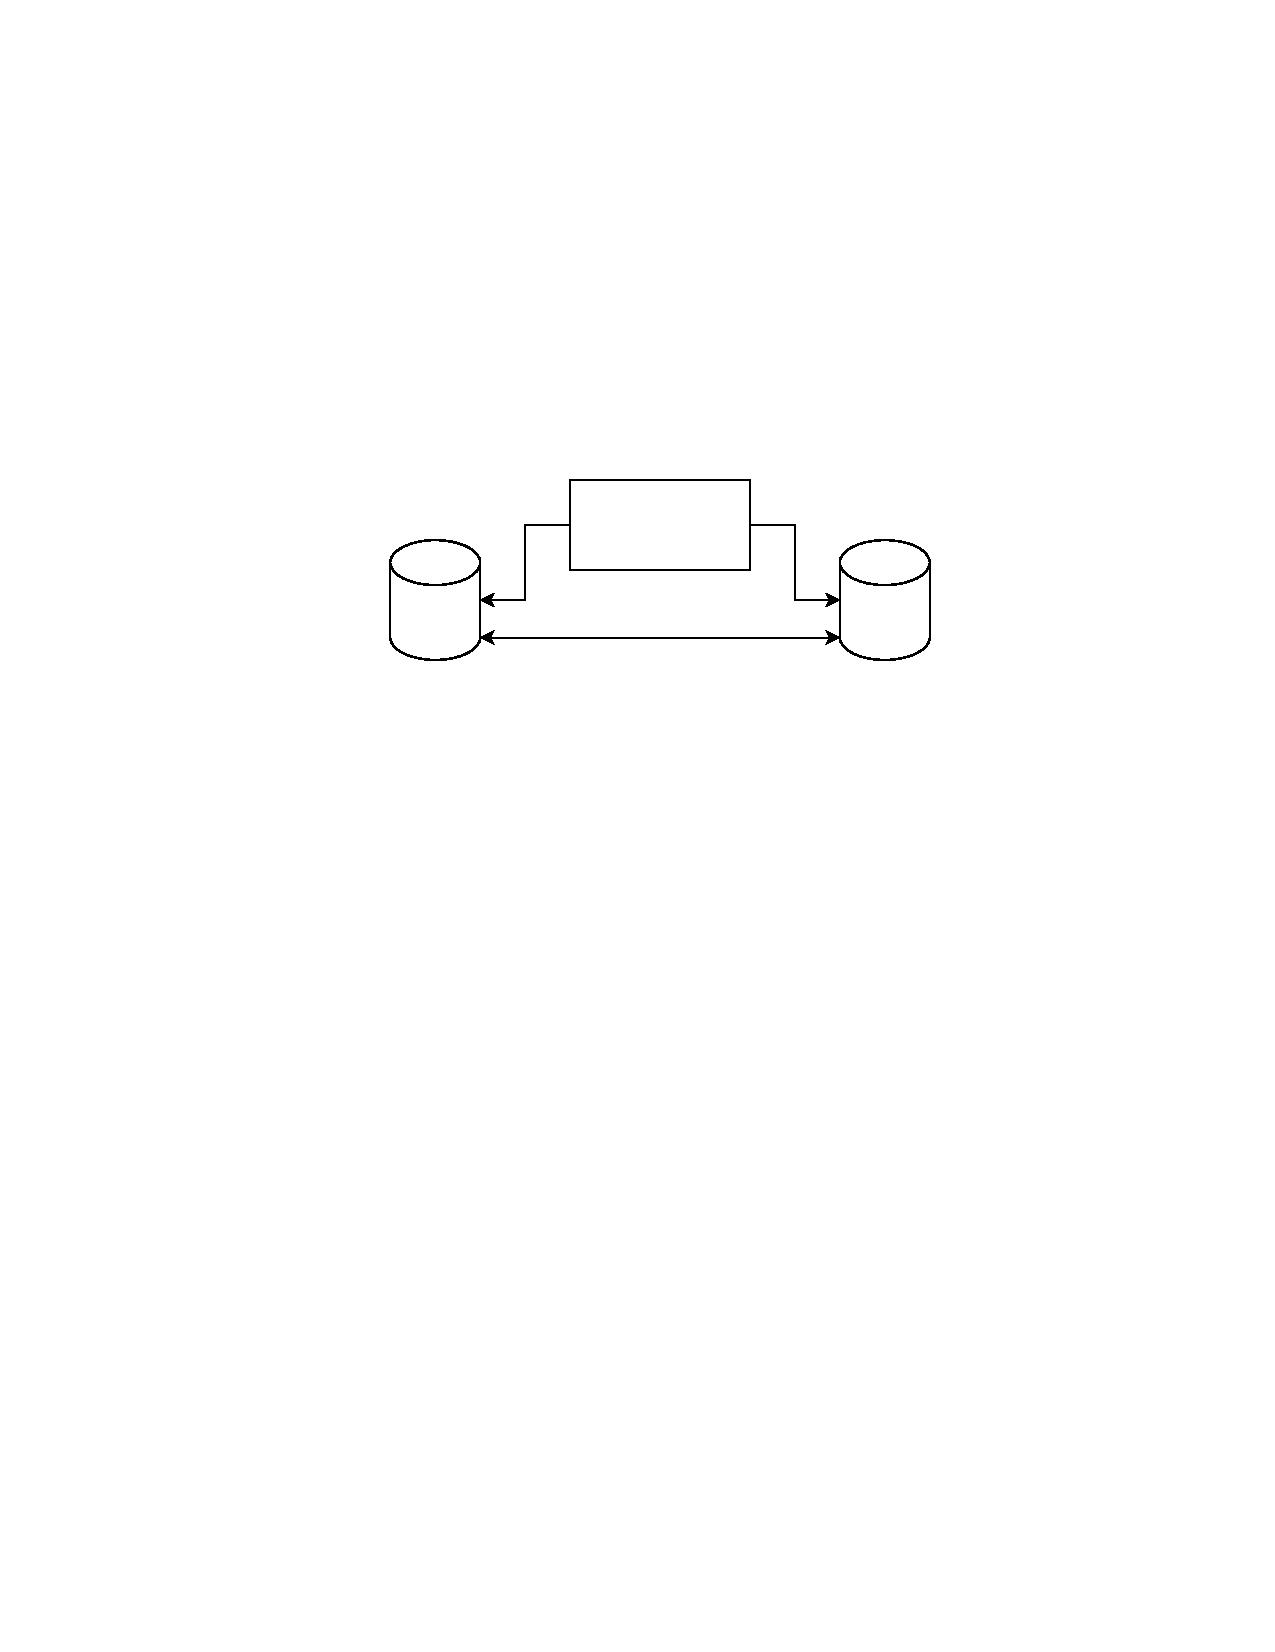
\includegraphics[width=1\textwidth]{diagram.pdf}
\end{figure}

\subsection{Základy}

Three.js prinieslo so sebou mnoho možností od ktorých sa odraziť a začať vyvíjať.
Na porovnanie na vytvorenie kocky s funkcionalitou rotácie kurzorom myši bez použitia three.js potrebovali niečo cez 200 riadkov kódu vrátane HTML, CSS, zatiaľ, čo pri three.js je toto číslo menšie ako 50.
Tieto čísla sú iba ilustračné, určite sú možnosti ako obidve zredukovať, slúžia pre demonštráciu ako nám vie three.js značne uľahčiť prácu a zvýšiť našu produktivitu.
Rozdielom pri používaný three.js oproti čistému WebGL je, že v three.js si nemusíme vytvárať 3D objekty ručne určovaním vektorov, vyberiete si funkciu na tvorbu objektu, ktorá toto poskladá za vás.

\subsection{3D Objekty}

Na začiatok treba spomenúť nejaké základy na prácu s 3D. Pri práci s budeme vytvárať mesh objekty.
“Mesh je všeobecnosti len, Sieť je vo všeobecnosti len skupina mnohouholníkov s niektorými súvisiacimi údajmi, ako je farba, ktorú vykresľujeme.” \cite{Graphics-openGL}
Tieto mesh objekty v three.js sa vytvárajú za pomoci geometrie a materiálu, ktorý môže predstavovať textúra, či farba.

\subsection{Zobrazenie}

Ešte sa ale musíme zastaviť pri jednom bode aby to všetko fungovalo. Aby sme vedeli vytvoriť takúto scénu, budeme potrebovať spojiť niekoľko častí.
Budeme potrebovať samotnú scénu, v našom prípade to bude reprezentovať okno prehliadača. Ďalej si vytvoriť kameru, bez nej by sme náš objekt asi horko ťažko hľadali.
“Aj napriek tomuto, pri spustení programu nebudeme schopný vidieť žiadnu zmenu. Je to preto, že v skutočnosti ešte nič nevykresľujeme. Na to potrebujeme to, čo sa nazýva kresliaca alebo animovaná slučka.” \cite{Three-js}

\subsection{Viac}

Tu to ale všetko nekončí. Naopak, otvára sa nám nová brána možností.  Ďalej vieme pridávať dynamickosť.
Pre vytvorenie pohybu rotácie takej kocky budeme potrebovať vytvoriť cyklus, ktorý bude postupne našej kocke meniť hodnotu.
Ľudské oko je dosť nedokonalé, a je ľahké ho oklamať.
Stačí viac ako dvanásť snímkov za sekundu a môže sa nám zdať, sa  sa nepozeráme ani na obrázky, ale vidíme pohyb.
Táto rýchlosť môže byť individuálna od problematiky.
Vo filmovom priemysle s menšou spotrebou vizuálnych efektov sa používa dvadsaťštyri snímkov, naopak pri filmoch s viacerými prvkami týchto efektov môžeme ísť do výšky až šesťdesiat.
Nám na webovej stránke bude stačiť  pohyb rýchlosťou medzi tridsať  a šesťdesiat snímkov za sekundu.
Ak by sme šli do menších čísel, mohlo by sa nám stať, že by sa pohyb nezdal byť taký plynulý.
Cyklus v JavaScripte vytvoríme funkciou requestAnimationFrame. V tomto cykle pridáme menšie číslo k starej hodnote rotácie na nami zvolenú os.
Treba si dávať pozor, ak to s hodnotami preženieme, naša scéna sa môže začať správať divne a zasekávať.

\section{Záver}

Je dôležité pochopiť základné koncepty, od ktorých sa už všetko neskôr odráža.
Taktiež  je dôležité si to v rámci pochopenia, vyskúšať v praxi. Neskôr sa náš vývoj bude hýbať smerom vpred.
Ako to už funguje v IT svete, veľa celkom na seba súvisí, preto je dôležité sa v niektorých orientovať, aby sme sa stali dobrými programátormi.

\bibliography{literatura}
\bibliographystyle{plain}
\end{document}
